\documentclass[12pt]{article}
\usepackage[english]{babel}
\usepackage[utf8]{inputenc}

%% Pointer to 'default' preamble
% pacakages and definitions

\usepackage{geometry}
\geometry{
	letterpaper, 
	portrait, 
	top=.75in,
	left=.8in,
	right=.75in,
	bottom=.5in		} 	% Page Margins
	
%% additional packages for nice things
\usepackage{amsmath} 	% for most math
\usepackage{commath} 	% for abs
\usepackage{lastpage}	% for page count
\usepackage{amssymb} 	% for therefore
\usepackage{graphicx} 	% for image handling
\usepackage{wrapfig} 	% wrap figures
\usepackage[none]{hyphenat} % for no hyphenations
\usepackage{array} 		% for >{} column characterisctis
\usepackage{physics} 	% for easier derivative \dv....
\usepackage{tikz} 		% for graphic@!
\usepackage{circuitikz} % for circuits!
\usetikzlibrary{arrows.meta} % for loads
\usepackage[thicklines]{cancel}	% for cancels
\usepackage{xcolor}		% for color cancels
\usepackage[per-mode=fraction]{siunitx} % for si units and num
\sisetup{group-separator = {,}, group-minimum-digits = 3} % additional si unit table functionality

\usepackage{fancyhdr} 	% for header
\usepackage{comment}	% for ability to comment out large sections
\usepackage{multicol}	% for multiple columns using multicols
\usepackage[framed,numbered]{matlab-prettifier} % matlab sytle listing
\usepackage{marvosym} 	% for boltsymbol lightning
\usepackage{pdflscape} 	% for various landscape pages in portrait docs.
%\usepackage{float}
\usepackage{fancyvrb}	% for Verbatim (a tab respecting verbatim)
\usepackage{enumitem}	% for [resume] functionality of enumerate
\usepackage{spreadtab} 	% for using formulas in tables}
\usepackage{numprint}	% for number format in spread tab
\usepackage{subcaption} % for subfigures with captions
\usepackage[normalem]{ulem} % for strike through sout

% for row colors in tables....
\usepackage{color, colortbl}
\definecolor{G1}{gray}{0.9}
\definecolor{G2}{rgb}{1,0.88,1}%{gray}{0.6}
\definecolor{G3}{rgb}{0.88,1,1}

% For table formatting
\usepackage{booktabs}
\renewcommand{\arraystretch}{1.2}
\usepackage{floatrow}
\floatsetup[table]{capposition=top} % put table captions on top of tables

% Caption formating footnotesize ~ 10 pt in a 12 pt document
\usepackage[font={small}]{caption}

%% package config 
\sisetup{output-exponent-marker=\ensuremath{\mathrm{E}}} % for engineer E
\renewcommand{\CancelColor}{\color{red}}	% for color cancels
\lstset{aboveskip=2pt,belowskip=2pt} % for more compact table
%\arraycolsep=1.4pt\def
\setlength{\parindent}{0cm} % Remove indentation from paragraphs
\setlength{\columnsep}{0.5cm}
\lstset{
	style      = Matlab-editor,
	basicstyle = \ttfamily\footnotesize, % if you want to use Courier - not really used?
}
\renewcommand*{\pd}[3][]{\ensuremath{\dfrac{\partial^{#1} #2}{\partial #3}}} % for larger pd fracs
\renewcommand{\real}[1]{\mathbb{R}\left\{ #1 \right\}}	% for REAL symbol
\newcommand{\imag}[1]{\mathbb{I}\left\{ #1 \right\}}	% for IMAG symbol
\definecolor{m}{rgb}{1,0,1}	% for MATLAB matching magenta
	
%% custom macros
\newcommand\numberthis{\addtocounter{equation}{1}\tag{\theequation}} % for simple \numberthis command

\newcommand{\equal}{=} % so circuitikz can have an = in the labels
\newcolumntype{L}[1]{>{\raggedright\let\newline\\\arraybackslash\hspace{0pt}}m{#1}}
\newcolumntype{C}[1]{>{\centering\let\newline\\\arraybackslash\hspace{0pt}}m{#1}}
\newcolumntype{R}[1]{>{\raggedleft\let\newline\\\arraybackslash\hspace{0pt}}m{#1}}

%% Header
\pagestyle{fancy} % for header stuffs
\fancyhf{}
% spacing
\headheight 29 pt
\headsep 6 pt

%% Header
\rhead{Thad Haines \\ Page \thepage\ of \pageref{LastPage}}
\chead{Comparison of PST Versions \\ `Extended' Term Simulation  }
\lhead{Research \\ 08/06/20}

\usepackage[hidelinks]{hyperref} % allow links in pdf
\usepackage{setspace}
\usepackage{multicol}
\begin{document}
\onehalfspacing
\paragraph{Scenario} \begin{center}
\begin{minipage}{.47\linewidth}
\centering
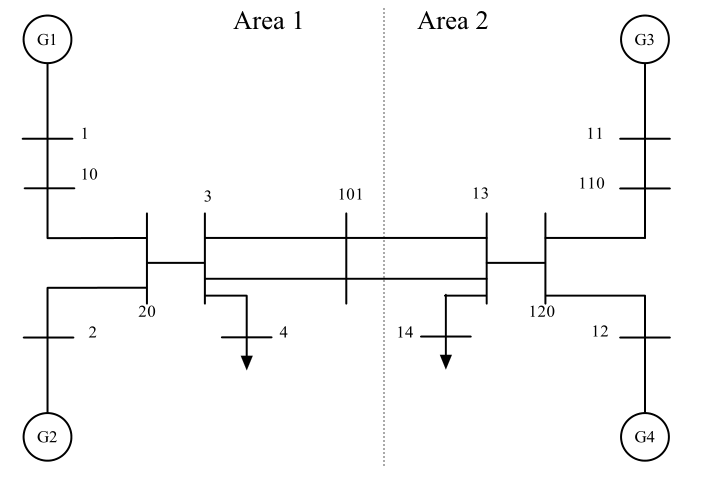
\includegraphics[width=\linewidth]{sysOneLineAreas}
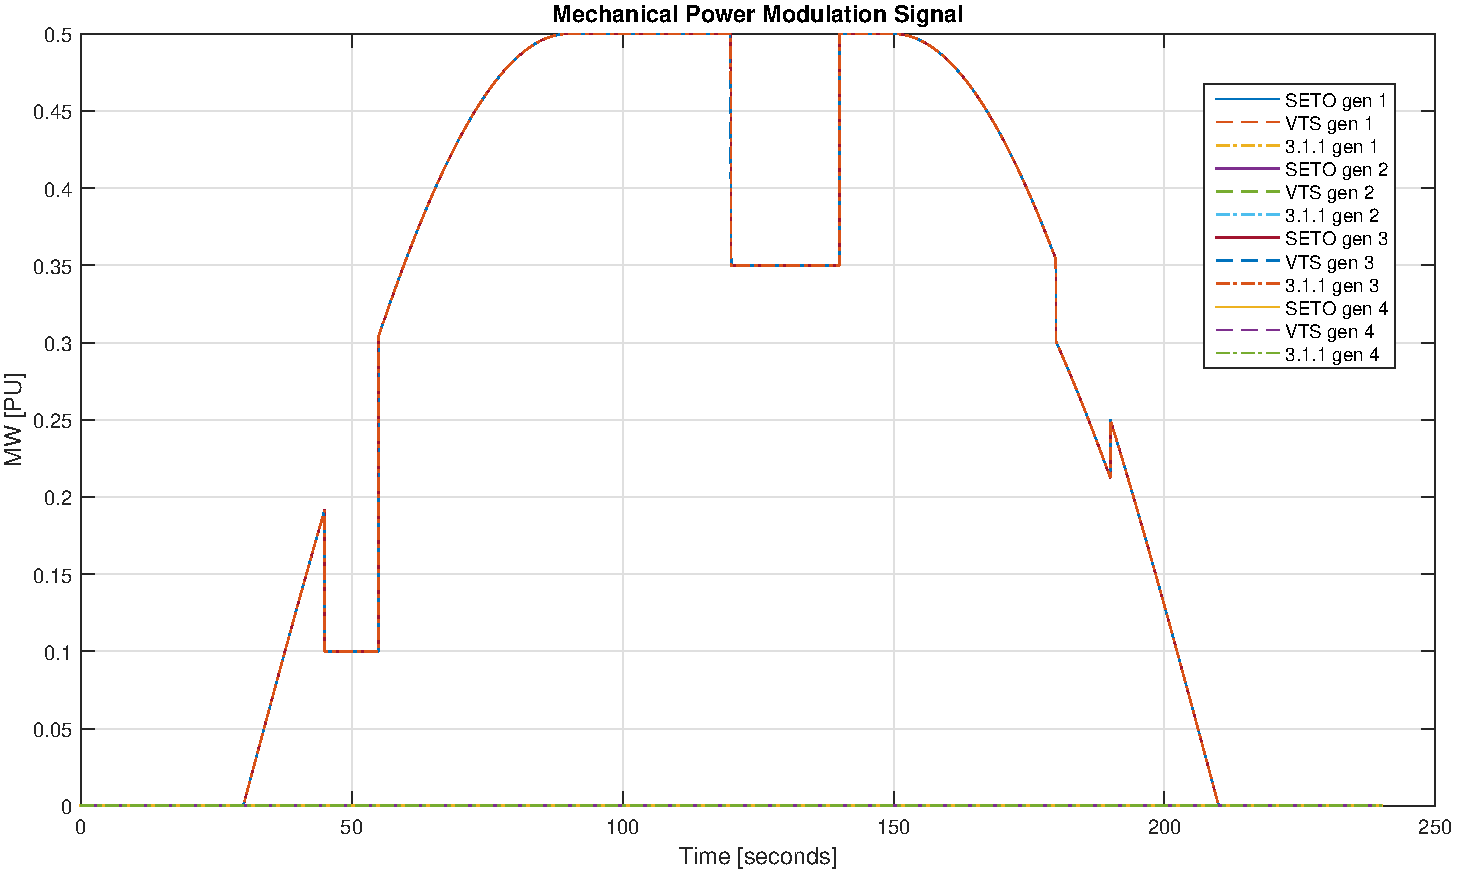
\includegraphics[width=.8\linewidth]{verPmSig}
\end{minipage} %
\begin{minipage}{.47\linewidth}
\begin{itemize}
\footnotesize
\itemsep 0em
\item Kundur  4 machine system packaged with PST
\item Constant Z load model
\item System has governors, exciters, and PSS.
\item Governor of generator being perturbed by pm\_sig removed
\item Perturbance was meant to mimic a solar ramp with various situations of cloud cover:\\
(larger plot of pm\_sig on Page 6)
\begin{Verbatim}[fontsize=\scriptsize]
% time [seconds]
% 0-30      - no action
% 30-90     - ramp up 0.5 PU (50 MW)
% 90-150    - hold peak
% 150-210   - ramp down 0.5 PU (50 MW)
% 210-240   - no action

% cloud cover events
% 45-55 - 20% max gen (generation of 0.1 PU)
% 120-140 - 30% cover (generation reduction to 70%)
% 180-190 - 15% cover (generation reduction to 85%)
\end{Verbatim}
\end{itemize}
\end{minipage}

\end{center}

\paragraph{Summary} 
\begin{enumerate}
\item The SETO version is 3.65 times faster than PST 3.1.1.
\item Using variable time steps allows for a speed up of 14.84 over PST 3.1.1.
\item Results from all simulations are very similar.
\item Without creating an explicit time block at the beginning of an event, VTS events may not occur at the exact time they are programmed.
\item VTS reduces logged data size by $\approx$4 times compared to the SETO version.
\end{enumerate}


\begin{table}[!ht]
\resizebox{\linewidth}{!}{

	\begin{tabular}{@{} L{1.75cm} 
	R{2cm} R{2cm}  R{2cm} R{1.5cm} R{0.75cm} R{0.75cm} R{1.5cm} R{2cm} R{2cm}@{}} 	
		\toprule % @ signs to remove extra L R space
		\footnotesize % this will affect the table font (makse it 10pt)
		\raggedright % for non justified table text

	&	\multicolumn{3}{c}{Step Size [seconds]}					&		&	\multicolumn{2}{c}{Solutions Per Step}			&		&		&		\\	
\shortstack{PST\\Version}	&	Max.	&	Min.	&	Ave.	&	Total Steps	&	Ave.	&	Max.	&	Total Slns.	&	Sim. Time	&	Speed Up	\\ \midrule	
3.1.1	&	4.00E-03	&	4.00E-03	&	4.00E-03	&	59,975	&	2	&	2	&	119,950	&	916.24	&	1.00	\\	
SETO	&	4.00E-03	&	4.00E-03	&	4.00E-03	&	59,975	&	2	&	2	&	119,950	&	250.82	&	3.65	\\	
VTS	&	2.32E+01	&	2.68E-04	&	2.58E-02	&	9,315	&	2	&	97	&	17,006	&	61.73	&	14.84	\\	
																				\bottomrule
	\end{tabular}
	}%end resize box
	
\paragraph{NOTE}
\begin{itemize}
\item VTS is still `experimental' and not completely validated/verified.
\item Related files are on github in the \href{https://github.com/thadhaines/MT-Tech-SETO/tree/master/PST/0-examples/extendedTerm}{MT-Tech-SETO\textbackslash PST\textbackslash 0-examples\textbackslash extendedTerm} folder.
\end{itemize}


\end{table}
\begin{comment}
\paragraph{Observations of Note}
\begin{enumerate}[resume]
\item DONK!@~

\end{enumerate}

\end{comment}

\pagebreak
% fixed: 8749 steps i.e., 17498 network solutions 

%>> compareVTSandFTS
%VTS time: 15.8579
%fixed time: 57.4479
 

\subparagraph{Plotted Results - Step Size / Number of Solutions Comparison} \ \\
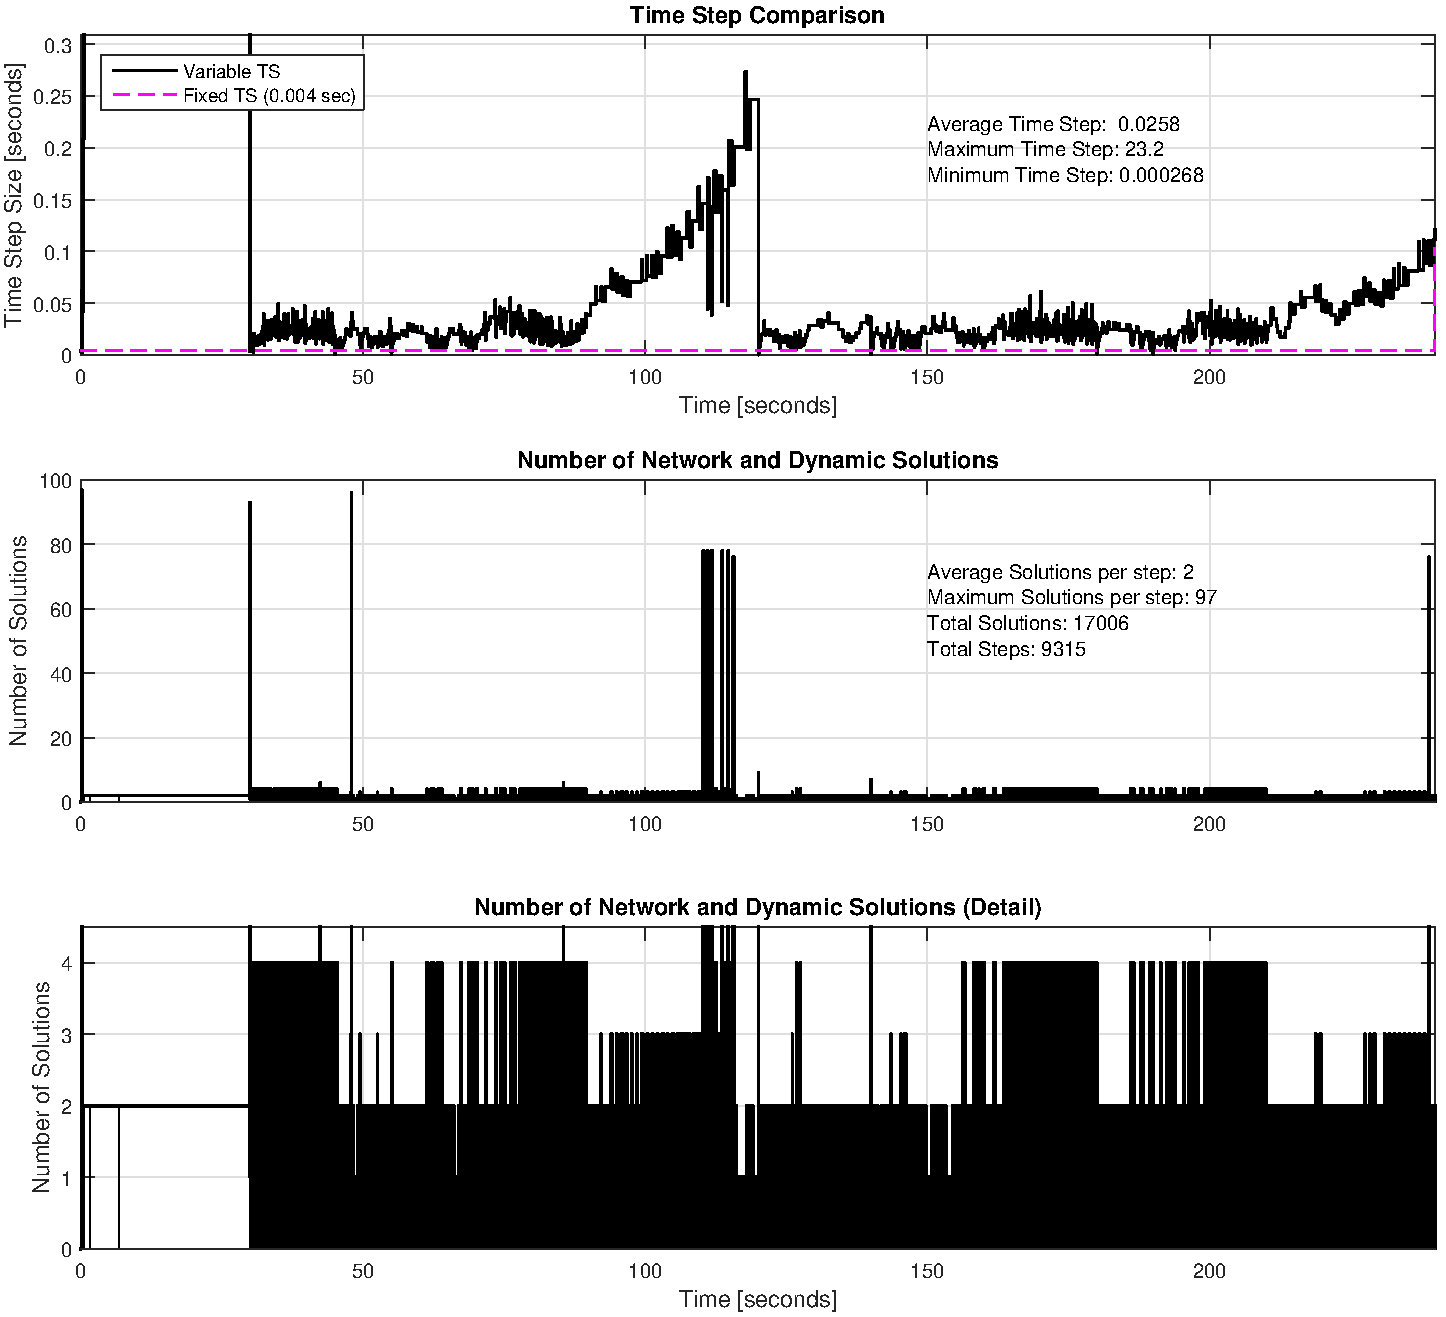
\includegraphics[width=\linewidth]{verSteps}

NOTE: Initial time steps before t=30 are much larger than the other time steps (multiple seconds) and are plotted off the axis.

\pagebreak
\subparagraph{Plotted Results - Various Comparisons} \ \\
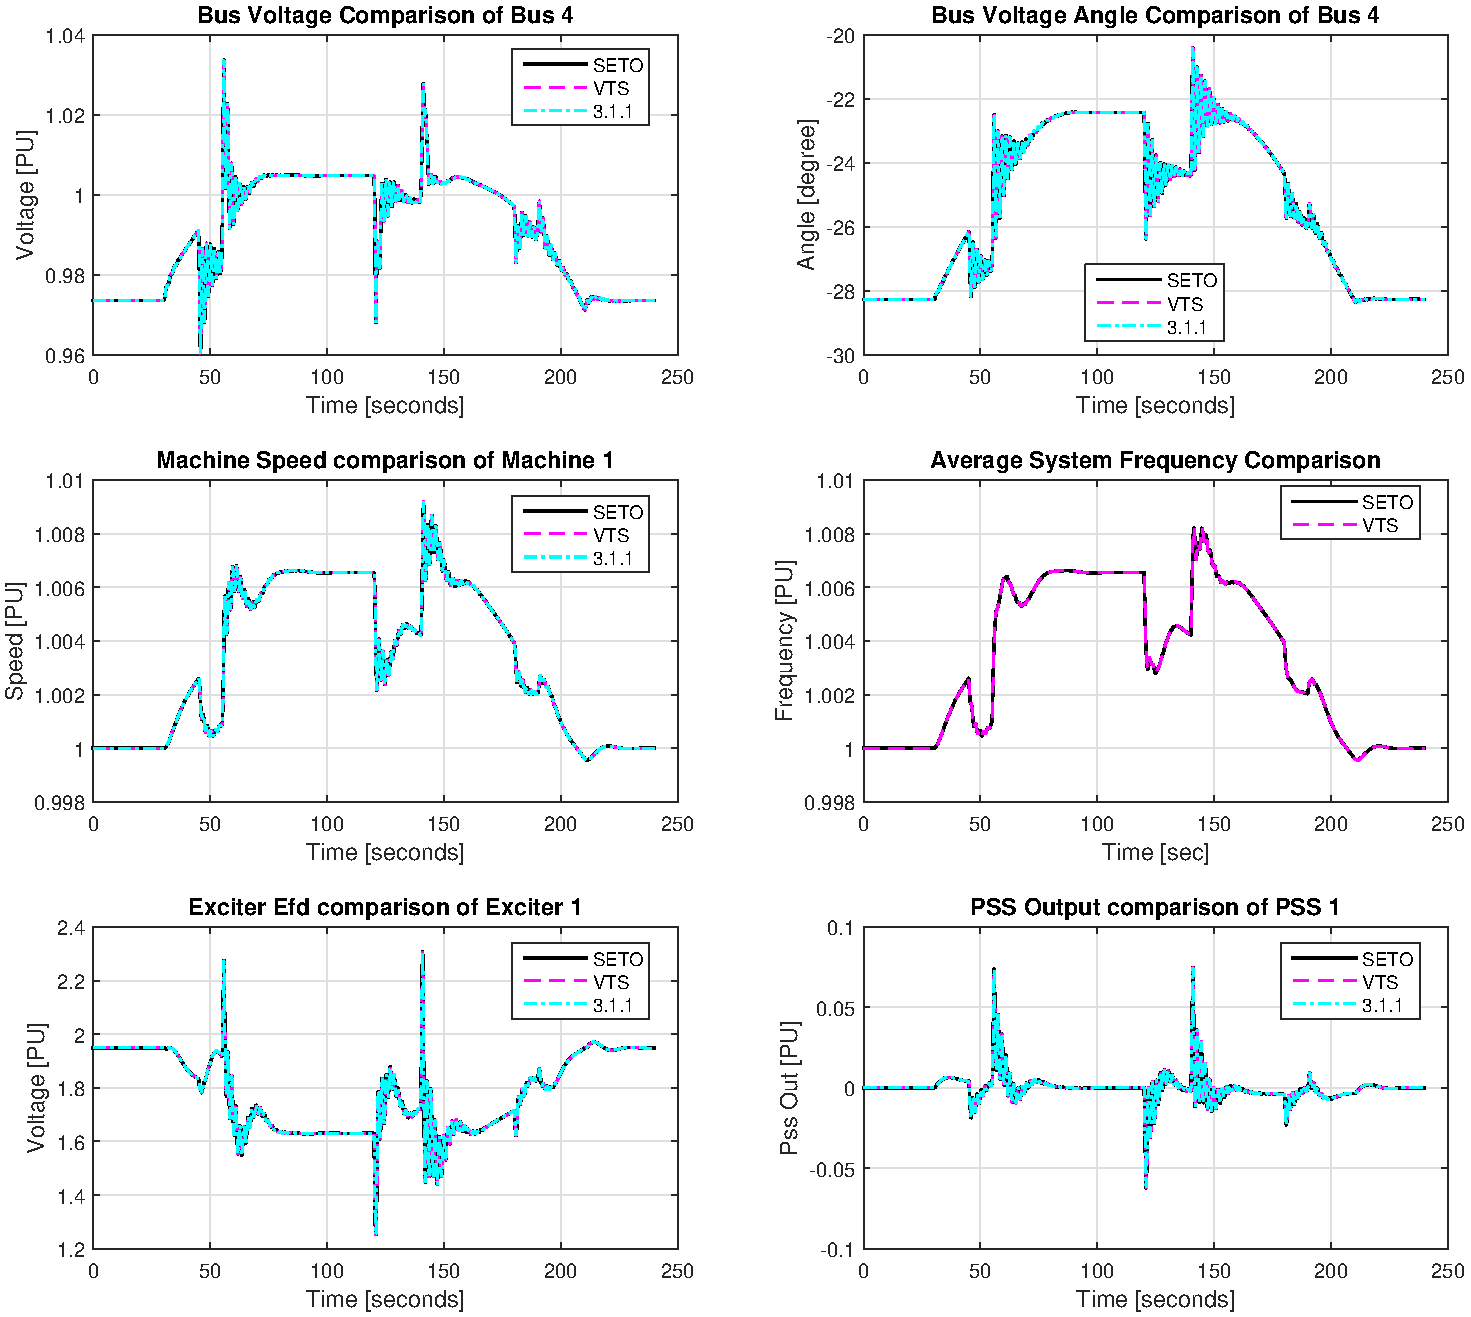
\includegraphics[width=\linewidth]{verComp}

NOTE: 3.1.1 does not calculate average system frequency.

\pagebreak
\subparagraph{Plotted Results - Various Comparisons - Detail 1} \ \\
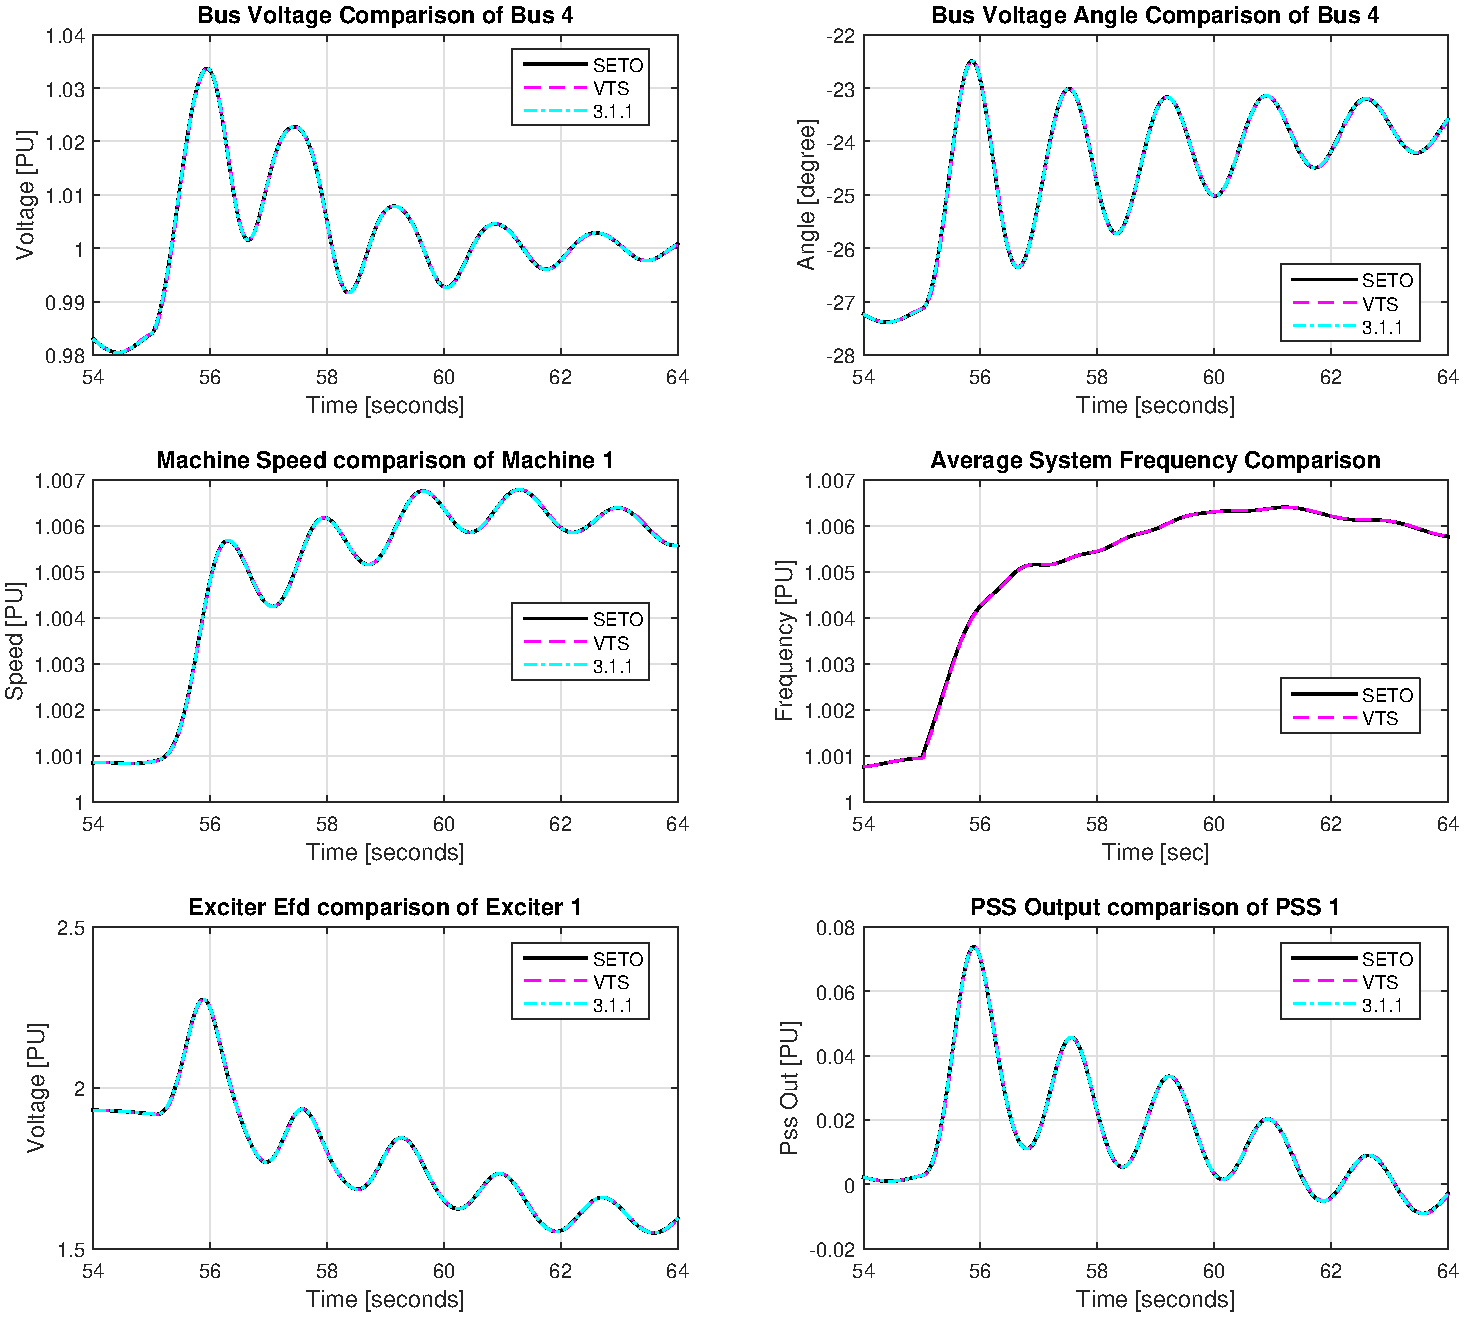
\includegraphics[width=\linewidth]{verCompDetail1}

NOTE: 3.1.1 does not calculate average system frequency.

\pagebreak
\subparagraph{Plotted Results - Various Comparisons - Detail 2} \ \\
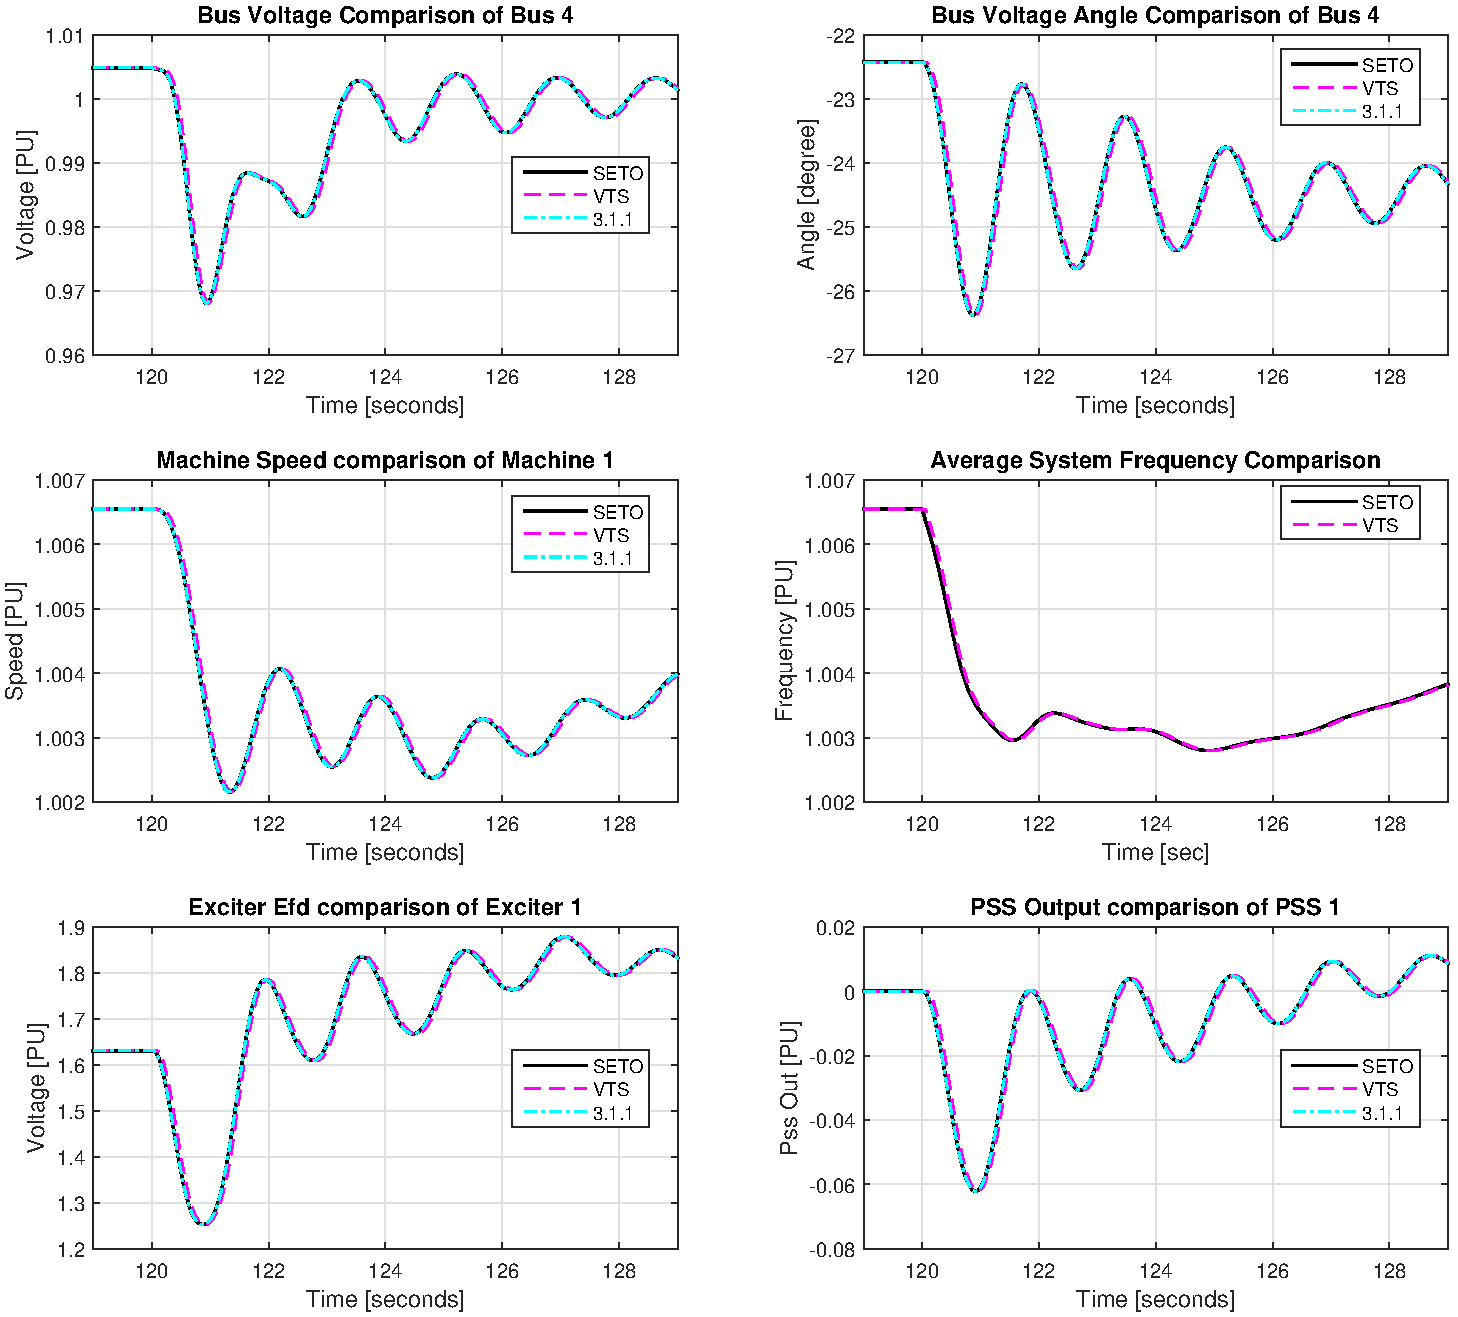
\includegraphics[width=\linewidth]{verCompDetail2}

NOTE: 3.1.1 does not calculate average system frequency.

VTS events may not occur at exact specified time due to the nature of variable time steps.

Breaks in the \verb|sw_con| can be created to account for this, however, the variance in time is often relatively small.


\pagebreak
\subparagraph{Plotted Results - Modulation Signal} \ \\
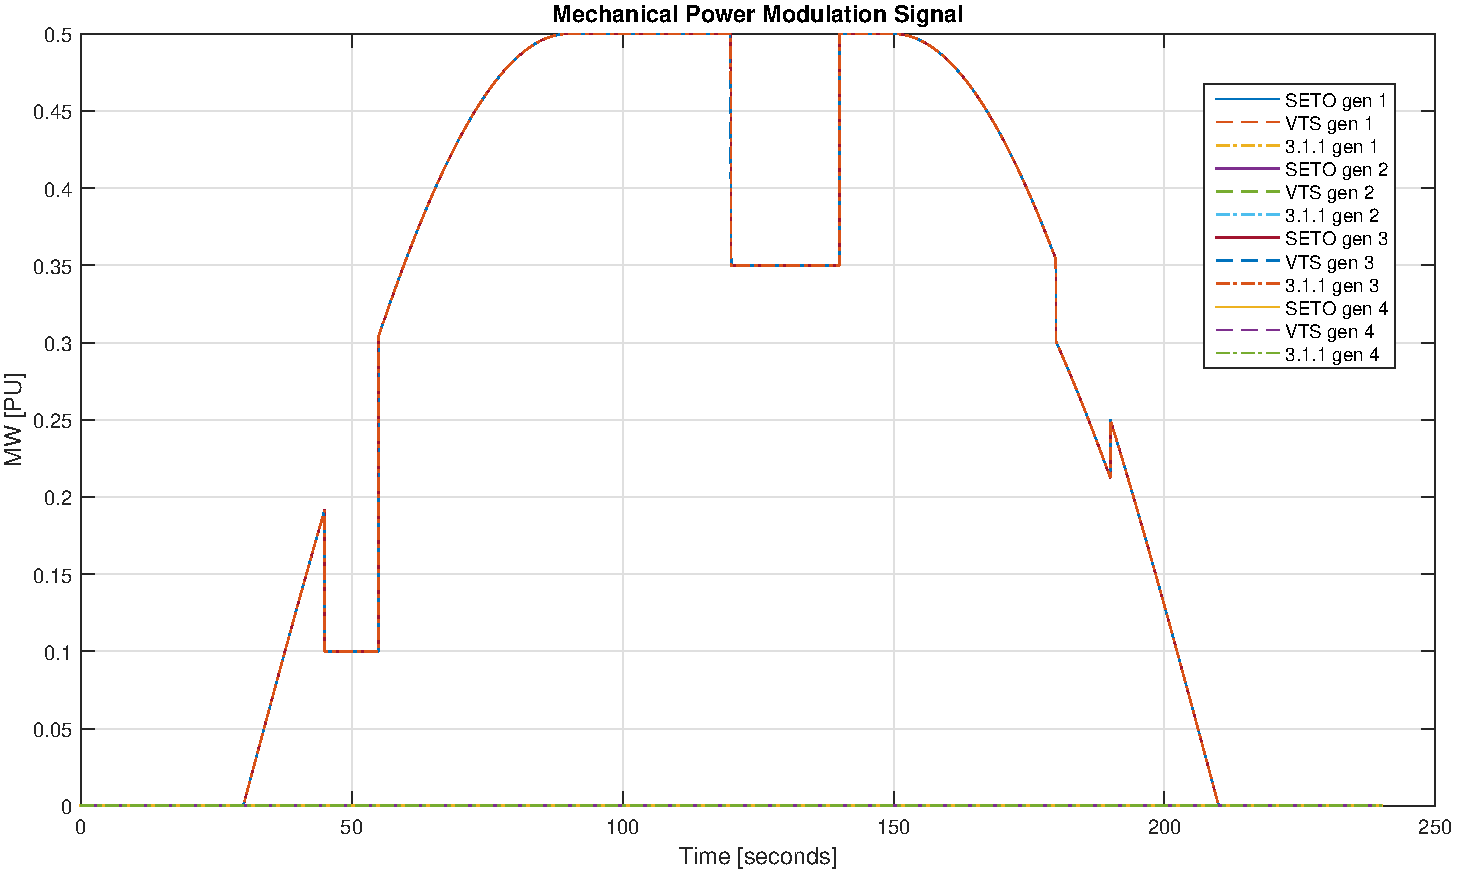
\includegraphics[width=\linewidth]{verPmSig}
\subparagraph{Plotted Results - Mechanical Power} \ \\
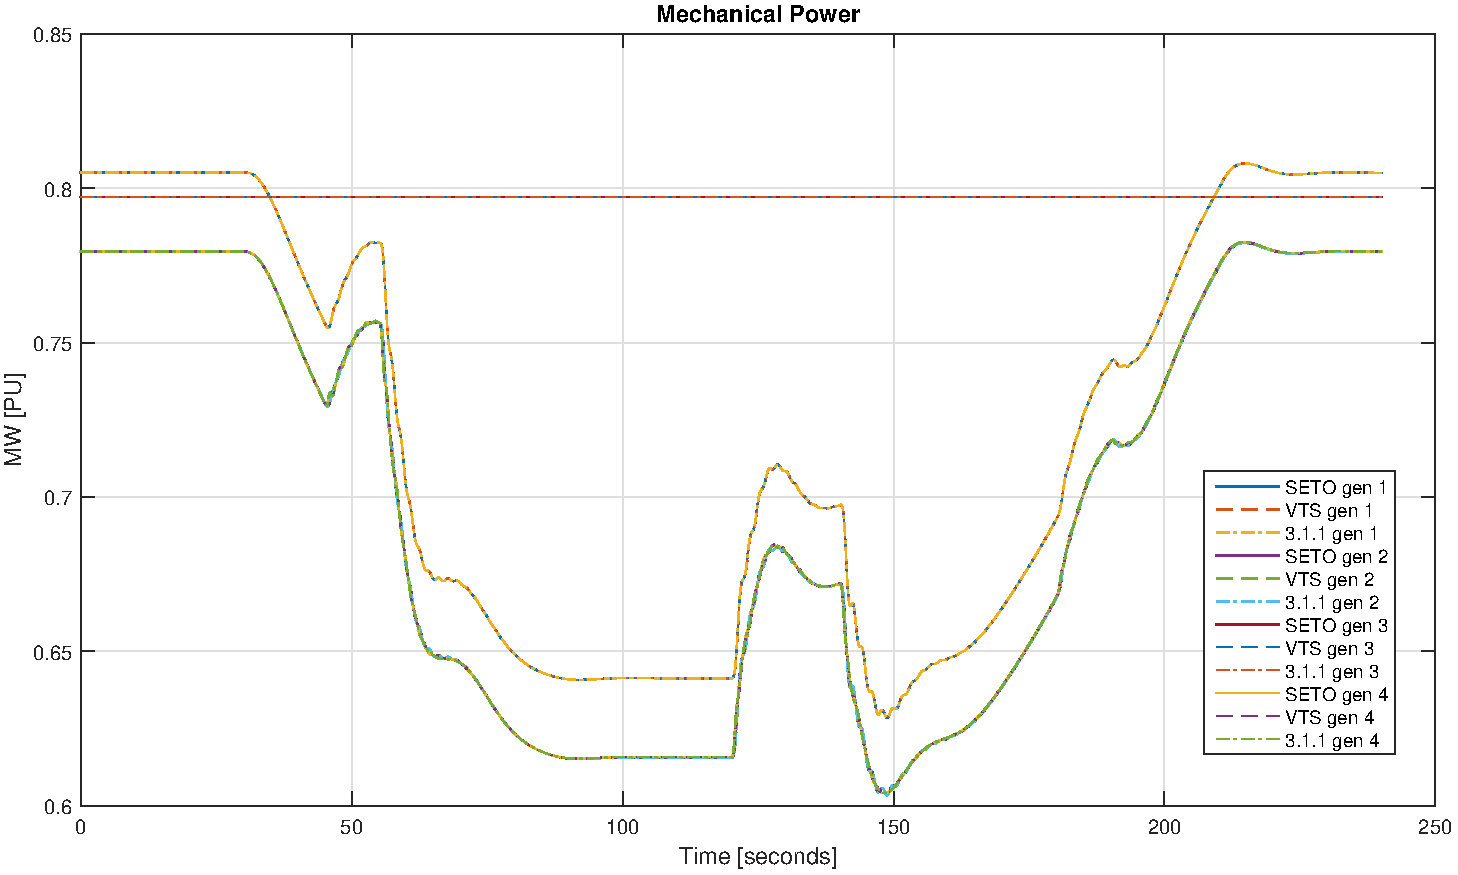
\includegraphics[width=\linewidth]{verPmech}
\subparagraph{Plotted Results - Electric Power} \ \\
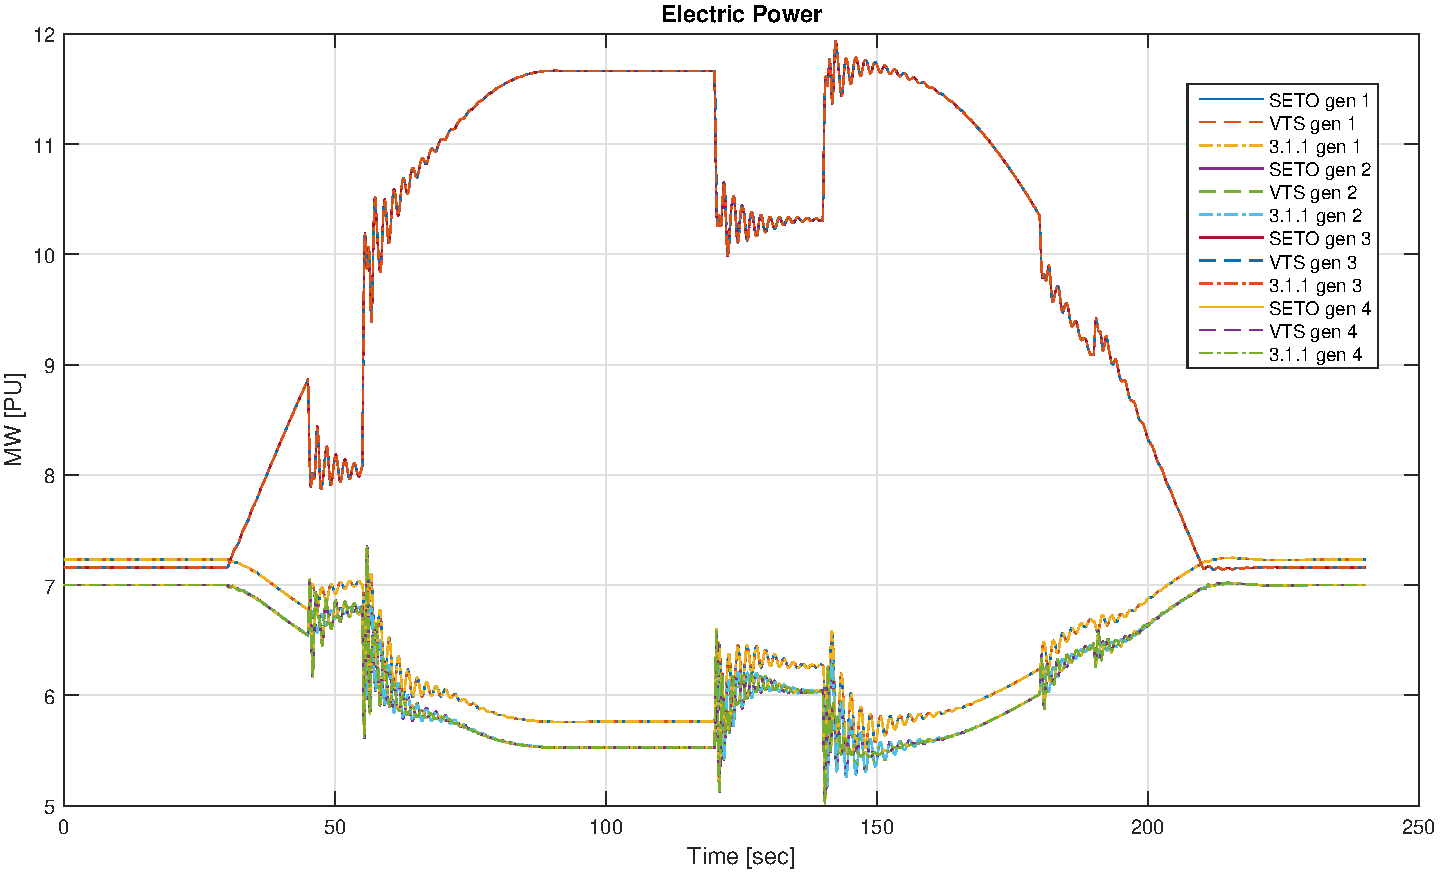
\includegraphics[width=\linewidth]{verPelect}

\subparagraph{Plotted Results - Electric Power - Detail} \ \\
Detail of generators 1, 2, and 5 from t= 140 to 150:

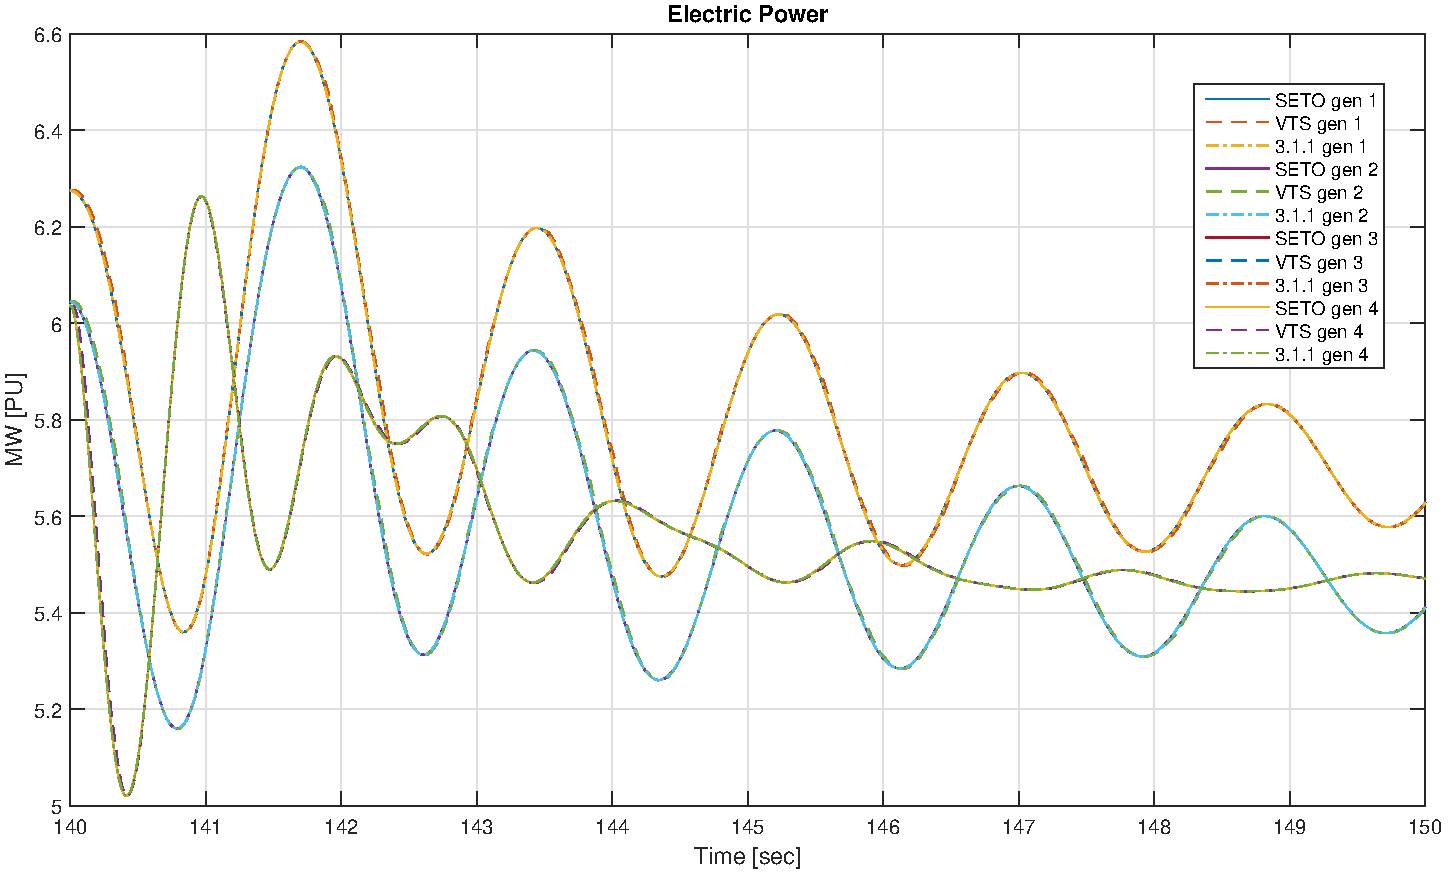
\includegraphics[width=\linewidth]{verPelectDetail}


\end{document}
